Il pattern architetturale applicato alla componente server è la \textit{Layered Architecture}. \\
Si è scelto tale pattern in quanto la componente server risulta troppo complessa per essere destrutturata dovendo gestire i servizi di: anagrafica unità, anagrafica utente, gestione mappa, calcolo percorsi unità e gestione delle interfacce grafiche.\\
Inoltre, garantendo il principio di \glock{Separation of Concerns} tipico di tale architettura, diverse squadre potranno lavorare su diversi layer autonomamente.
Di seguito viene illustrato il diagramma dei package. Si noti che le dipendenze procedono in un'unica direzione senza creare cicli. Si noti, inoltre, che il sistema dipende dalla classe \textbf{Position} in ogni suo punto in quanto, trattando problematiche legate al movimento di un'unità in una griglia, avere un tipo di dato che rappresenti due coordinate cartesiane risulta particolarmente utile.

\begin{figure}[H]
	\centering
	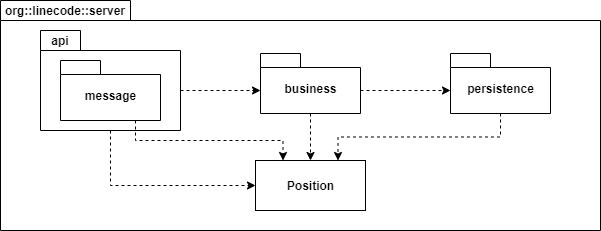
\includegraphics[width=12cm]{img/server_package.png}
	\caption{Server - Diagramma dei package}
\end{figure}

\begin{figure}[H]
    \centering
    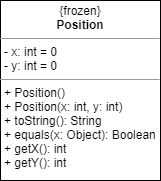
\includegraphics[width=4cm]{img/class_position.png}
    \caption{Server - Classe Position}
\end{figure}

\subsubsection{Messages}
È stato stabilito un formato standard di messaggi da e per UI e unità. Tali messaggi sono rappresentati come classi \glock{Java} e verranno scambiati con le altre componenti del prodotto in seguito alla loro serializzazione e deserializzazione in formato \glock{JSON}.\\
Ogni messaggio viene riferito tramite la propria interfaccia in modo da slegare il sistema dall'implementazione di tali messaggi.

\begin{landscape}
    \begin{figure}[H]
        \centering
        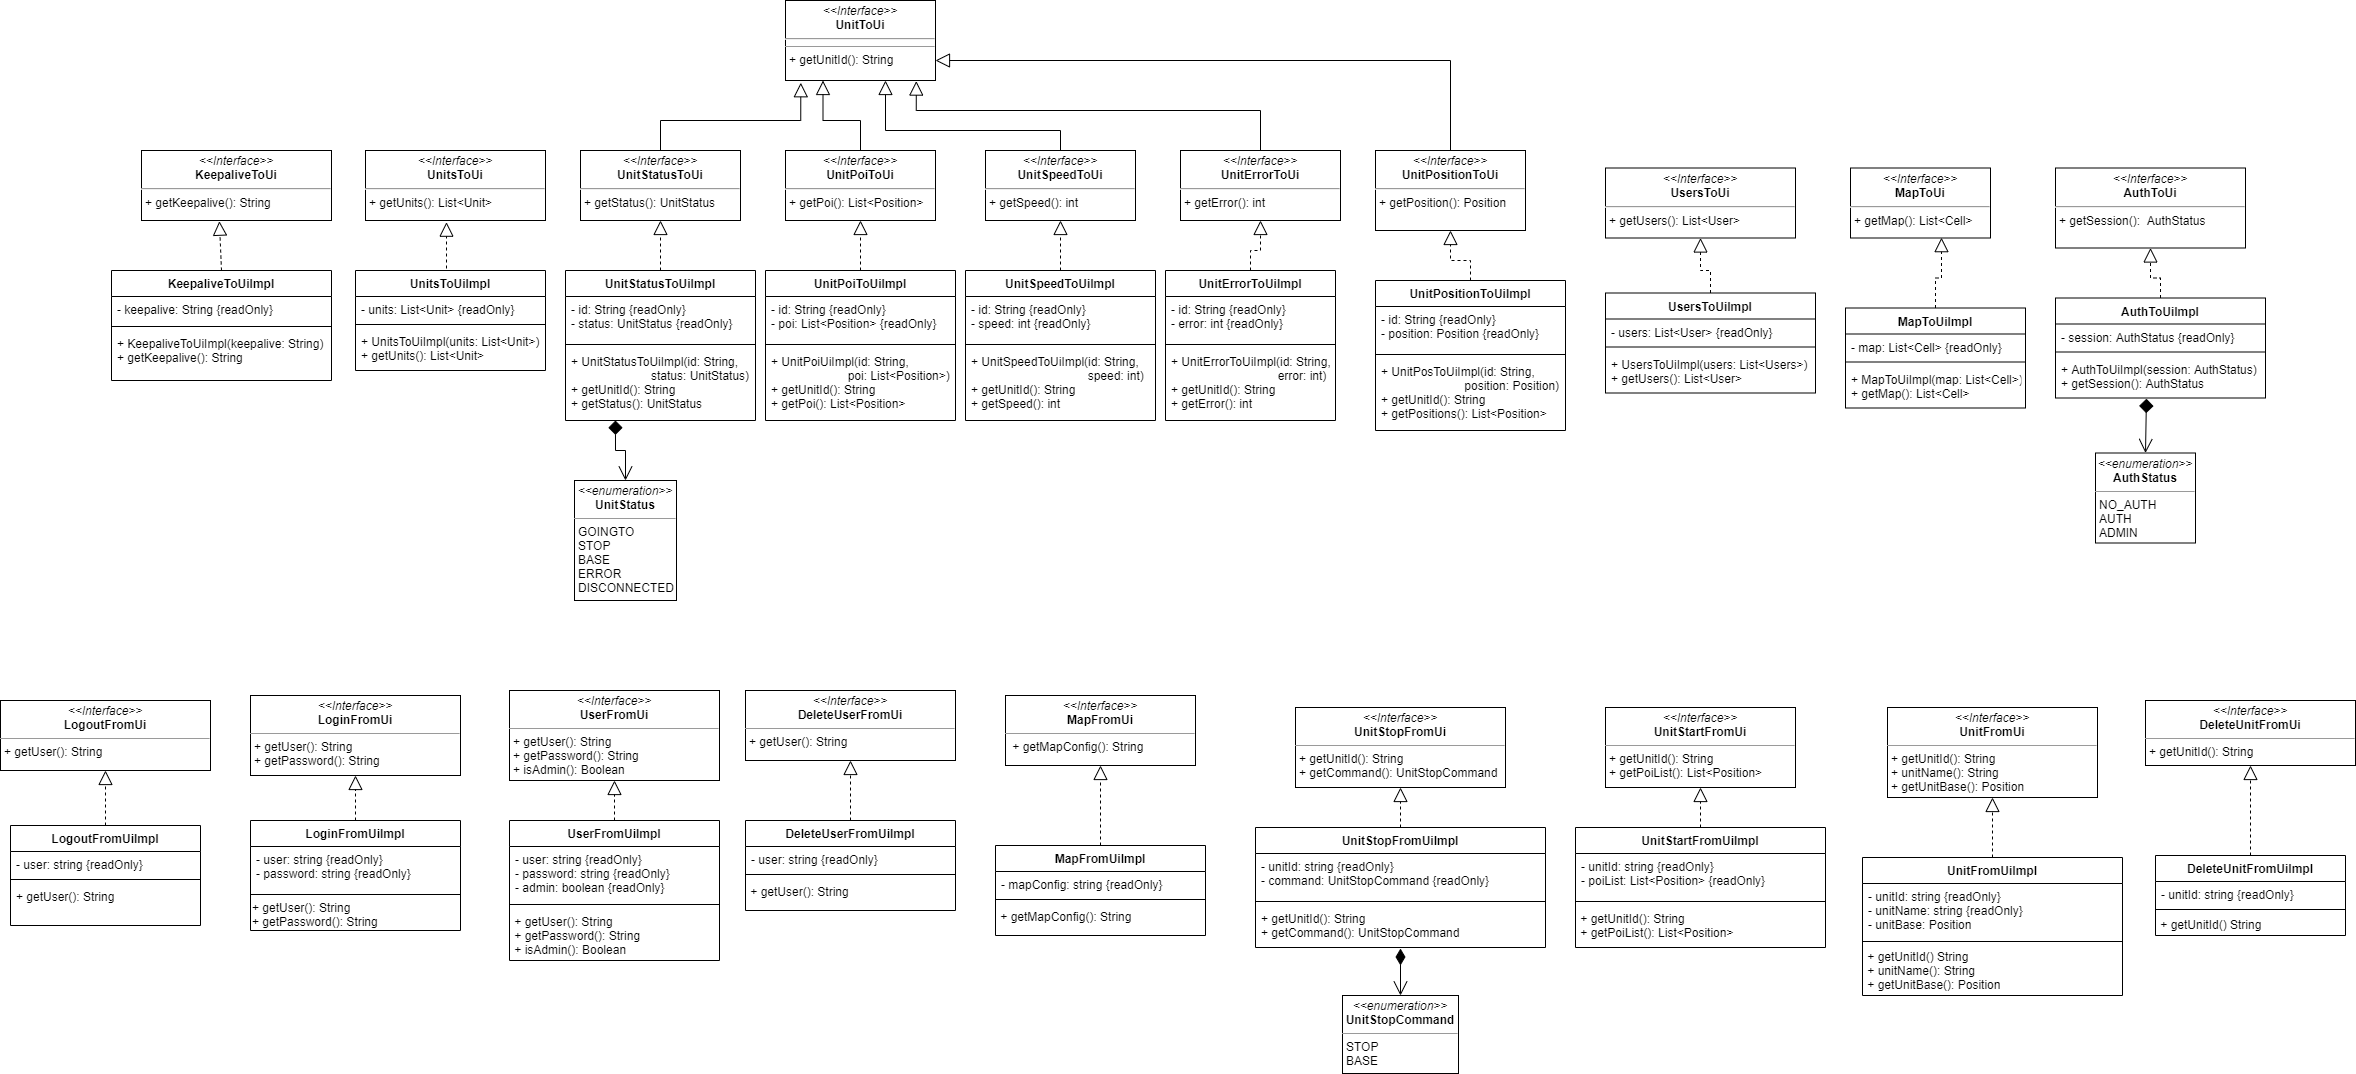
\includegraphics[width=23cm]{img/server_from_to_ui.png}
        \caption{Server - Messaggi da e per l'interfaccia}
    \end{figure}
\end{landscape}
\begin{landscape}
    \begin{figure}[H]
        \centering
        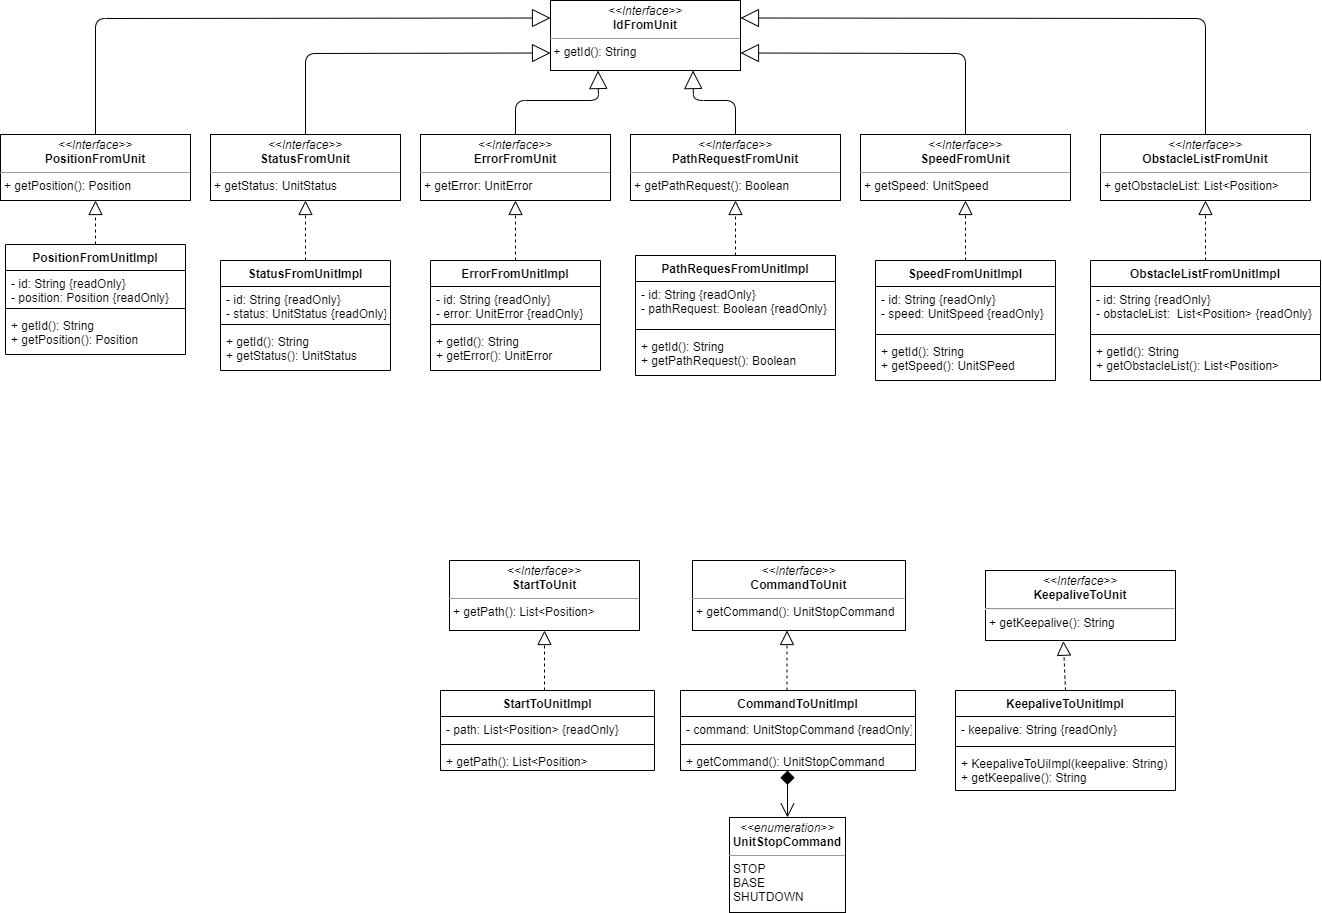
\includegraphics[width=22cm]{img/server_from_to_unit.png}
        \caption{Server - Messaggi da e per l'unità}
    \end{figure}
\end{landscape}

\subsubsection{API layer}
Qui troviamo i metodi che permettono la gestione della connessione alle altre componenti del sistema, e quindi anche l'invio e la ricezione di messaggi mediante opportune serializzazioni e deserializzazioni. Il tutto viene gestito dallo standard JRS 356 per i \glock{WebSocket} e da \glock{Jackson} per la (de)serializzazione.

\subsubsection{Business layer}
Qui troviamo la logica per l'elaborazione dei dati. Le informazioni scendono in questo layer tramite chiamata a funzione da parte dell'API layer su opportune interfacce. I prodotti dell'elaborazione vengono riportati nel layer superiore tramite oggetto ritornato dai metodi oppure, quando l'oggetto chiamante non è lo stesso che deve ricevere quanto ritornato, tramite l'emissione di opportuni segnali che verranno intercettati dal layer sovrastante secondo una logica \glock{signal/slot} simile alla libreria grafica \glock{Qt} fornita dalla libreria \glock{Sig4j}. Lo slot viene consegnato tramite chiamata a funzione dall'API layer alla costruzione dell'istanza Endpoint in modo che possa avvenire la connessione fra segnale e slot. In tal modo viene messo in atto un sistema di scambio dei messaggi "dal basso verso l'alto" mantenendo la direzione delle dipendenze in senso contrario.

\subsubsection{Persistence layer}
Qui troviamo le classi che permettono al Business layer di relazionarsi con il database indipendentemente dall'implementazione dello stesso grazie all'uso di opportune interfacce.

\begin{landscape}
    \begin{figure}[h!]
        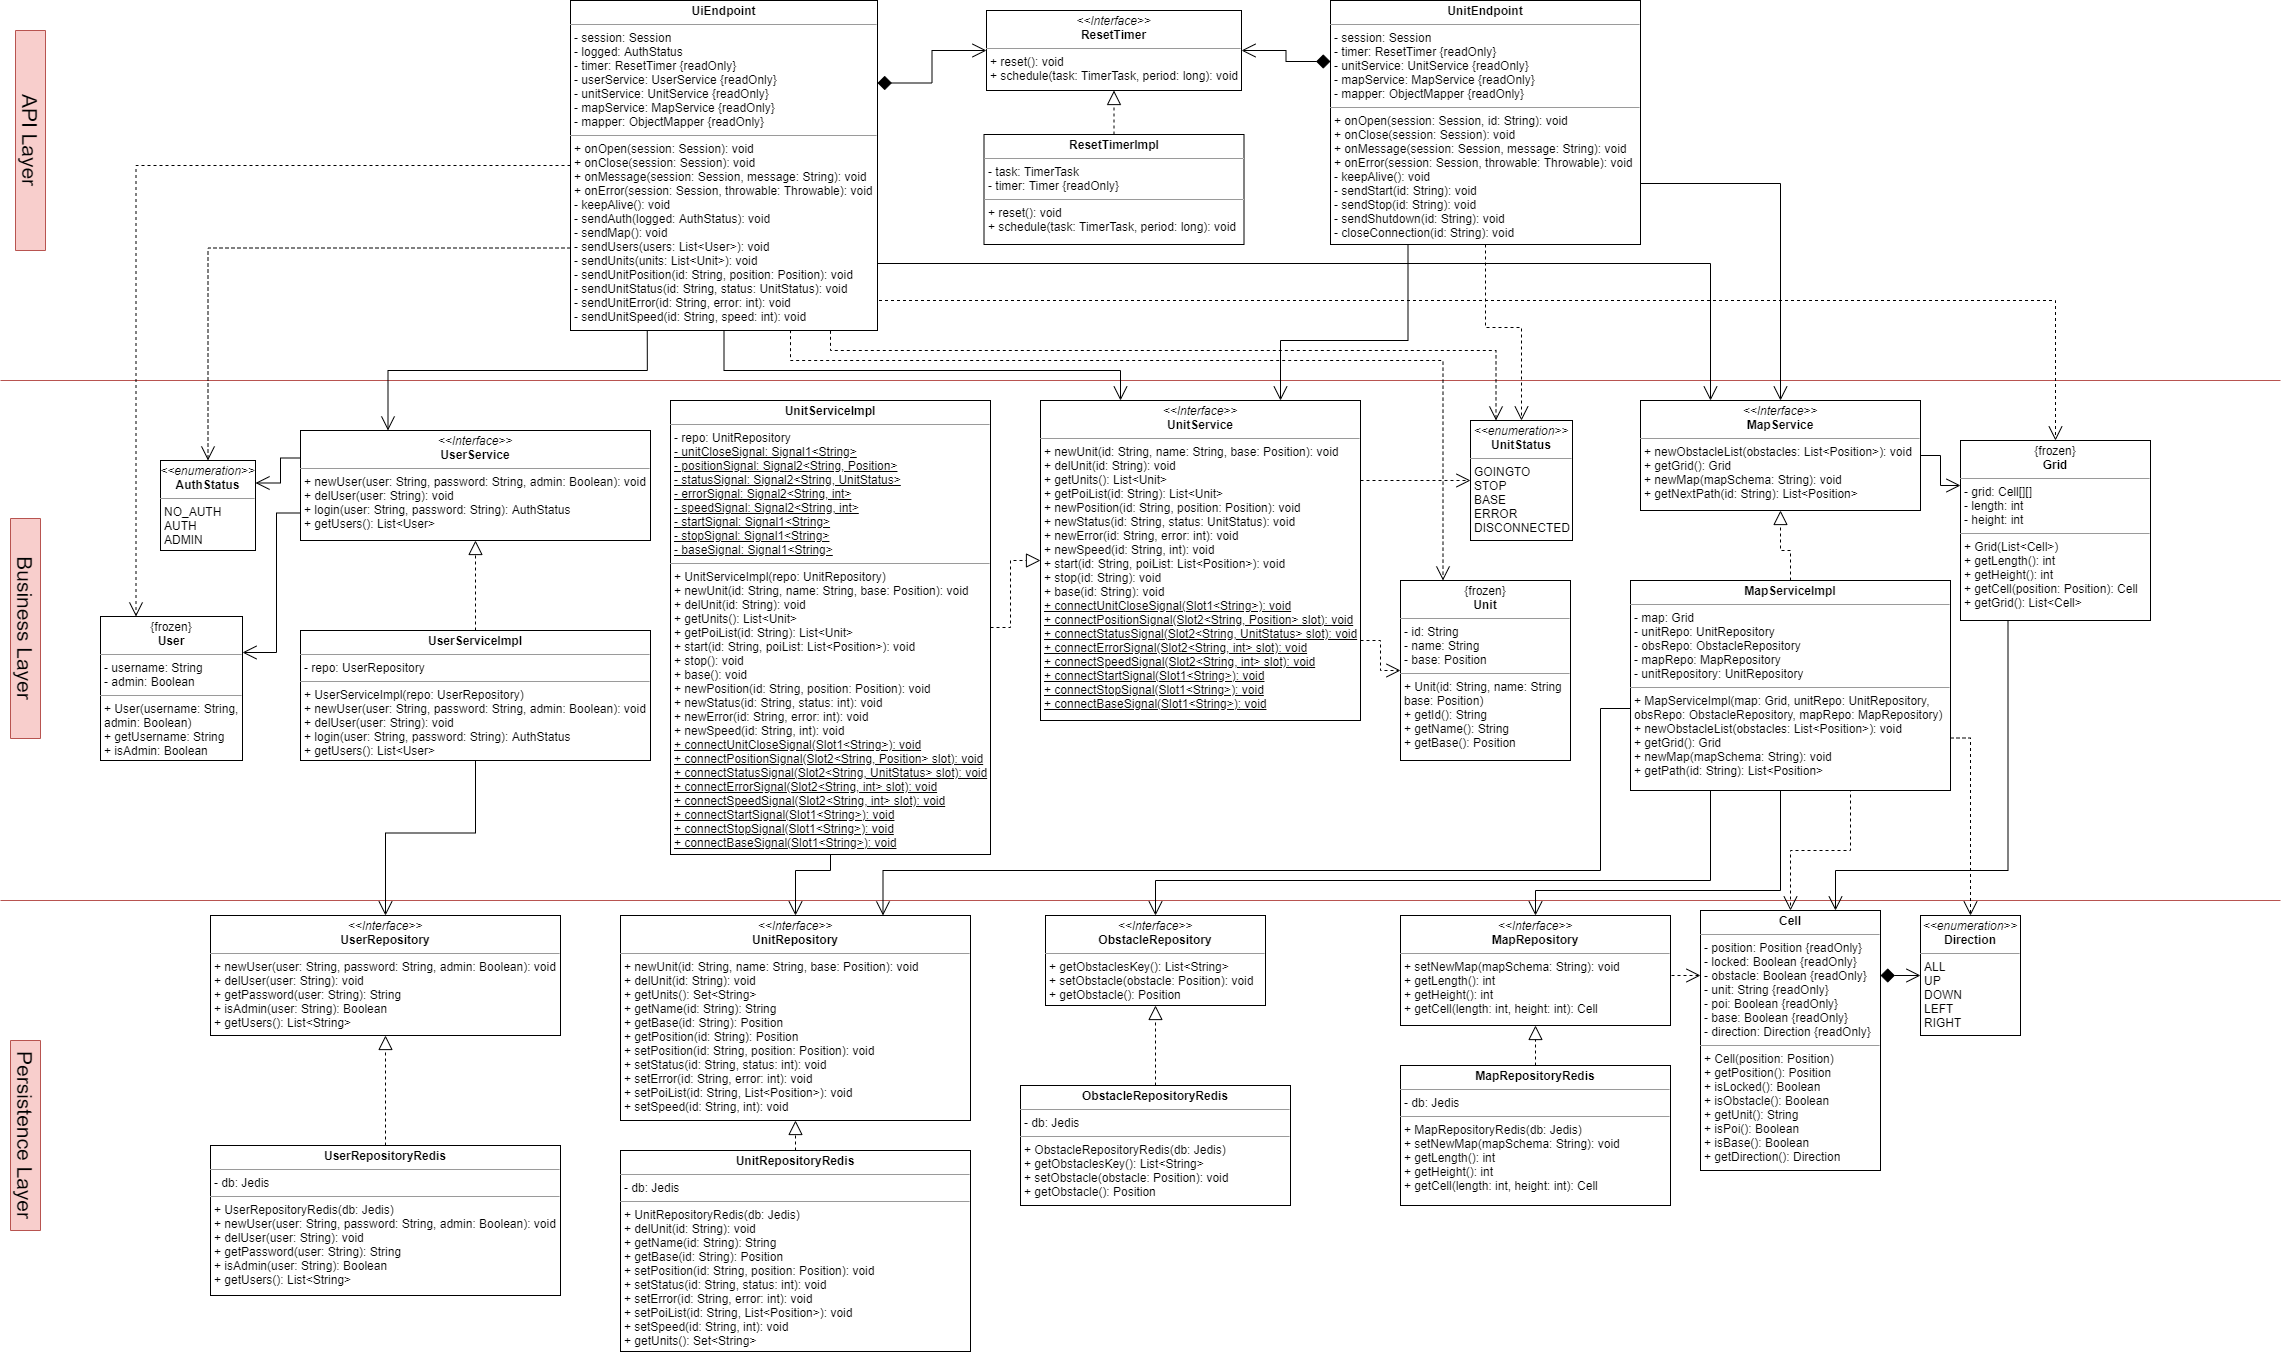
\includegraphics[width=26cm]{img/server_classi.png}
        \caption{Server - Diagramma delle classi}
    \end{figure}
\end{landscape}

\subsubsection{Database layer}
Per garantire le migliori performance al sistema e vista la quantità non eccessiva di dati, si è scelto \glock{Redis} come database essendo esso \glock{in-memory}. Non esistono diagrammi standard per rappresentarne la struttura dunque verranno di seguito elencate le strutture dati utilizzate:
\begin{itemize}
    \item SET con id delle unità (key = unit);
    \item HASH con dati e anagrafica delle unità (key = unit:[id\_unit]); campi dati:
    \begin{itemize}
        \item name;
        \item base\_x;
        \item base\_y;
        \item position\_x;
        \item position\_y;
        \item status;
        \item error;
        \item speed;
    \end{itemize}
    \item LIST con coordinate \glock{POI} da raggiungere per una specifica unità (key = poi:[id\_unit], valori = [coord\_x]:[coord\_y]);
    \item SET con username degli user (key = user);
    \item HASH con anagrafica degli user (key = user:[username]); campi dati:
    \begin{itemize}
        \item password;
        \item admin;
    \end{itemize}
    \item STRING con lunghezza tabella, asse x (key = length);
    \item STRING con altezza tabella, asse y (key = height);
    \item HASH con dati delle celle della mappa (key = cell:[coord\_x]:[coord\_y]); campi dati:
    \begin{itemize}
        \item position\_x;
        \item position\_y;
        \item locked;
        \item poi;
        \item base;
        \item direction;
    \end{itemize}
    \item SET con id intero incrementale degli ostacoli (key = obs);
    \item HASH con posizione dell’ostacolo e timestamp di rilevamento (key = obs:[obs\_id]); campi dati:
    \begin{itemize}
        \item position\_x;
        \item position\_y;
        \item timestamp.
    \end{itemize}
\end{itemize}

\begin{landscape}
    \subsubsection{Diagrammi di sequenza}
    Il seguente diagramma rappresenta il caso in cui l'interfaccia grafica invii al server una lista di \glock{POI}, che l'unità deve raggiungere.\\
    \begin{figure}[H]
        \centering
        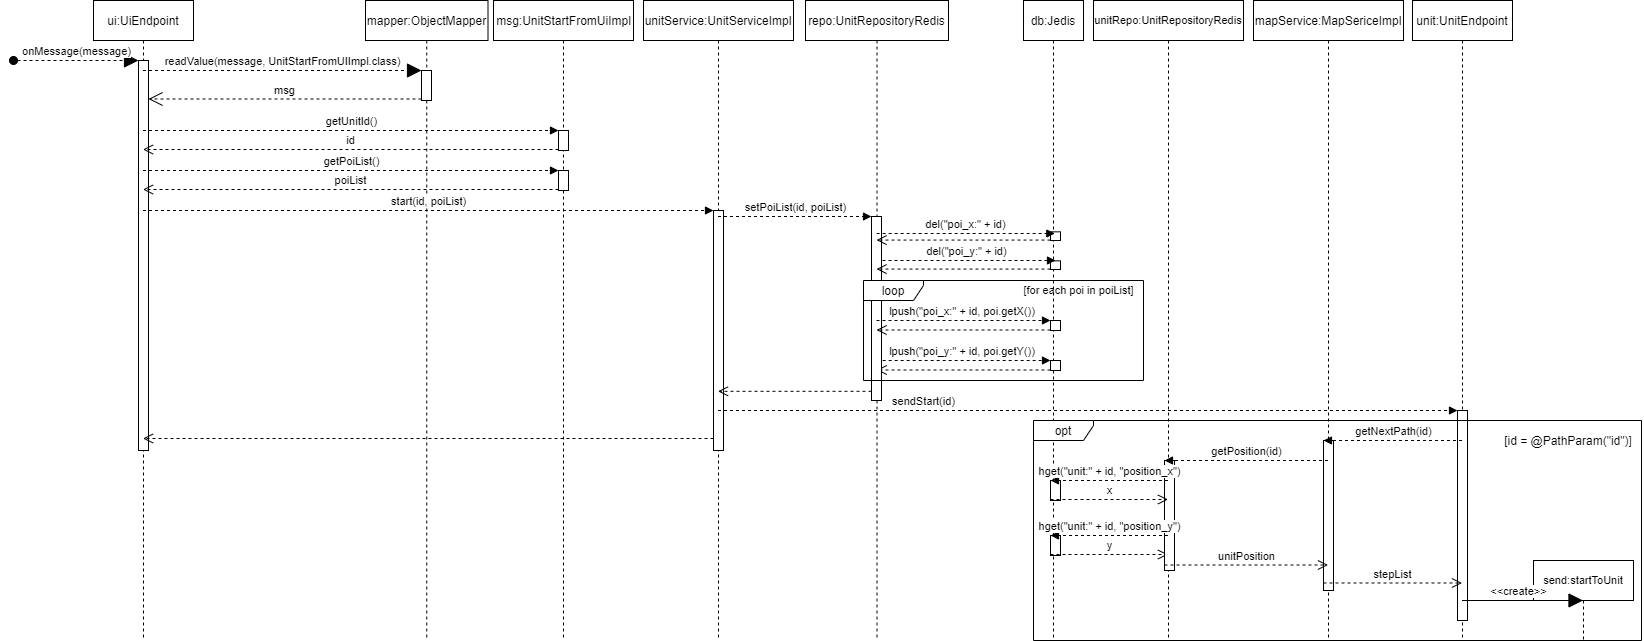
\includegraphics[width=25.7cm]{img/server_seq1.png}
        \caption{Server - UI invia una lista di \glock{POI} che l'unità deve raggiungere}
    \end{figure}
\end{landscape}

\newpage

\begin{landscape}
    Il seguente diagramma rappresenta il caso in cui un utente esegua il login dall'interfaccia grafica.
    \begin{figure}[H]
    	\centering
    	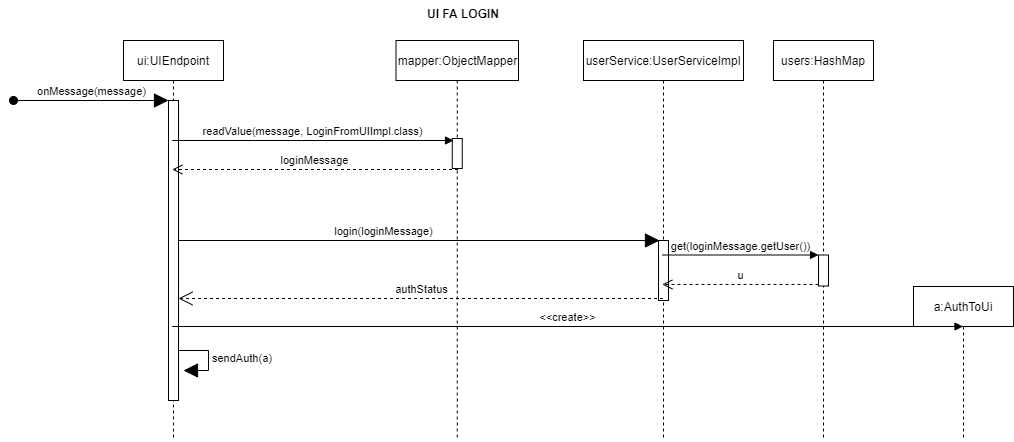
\includegraphics[width=25.7cm]{img/server_seq2.png}
    	\caption{Server - Richiesta di login da parte della UI}
    \end{figure}
\end{landscape}

\newpage

\begin{landscape}
    Il seguente diagramma rappresenta il caso in cui un utente elimini un'unità registrata.
    \begin{figure}[H]
        \centering
        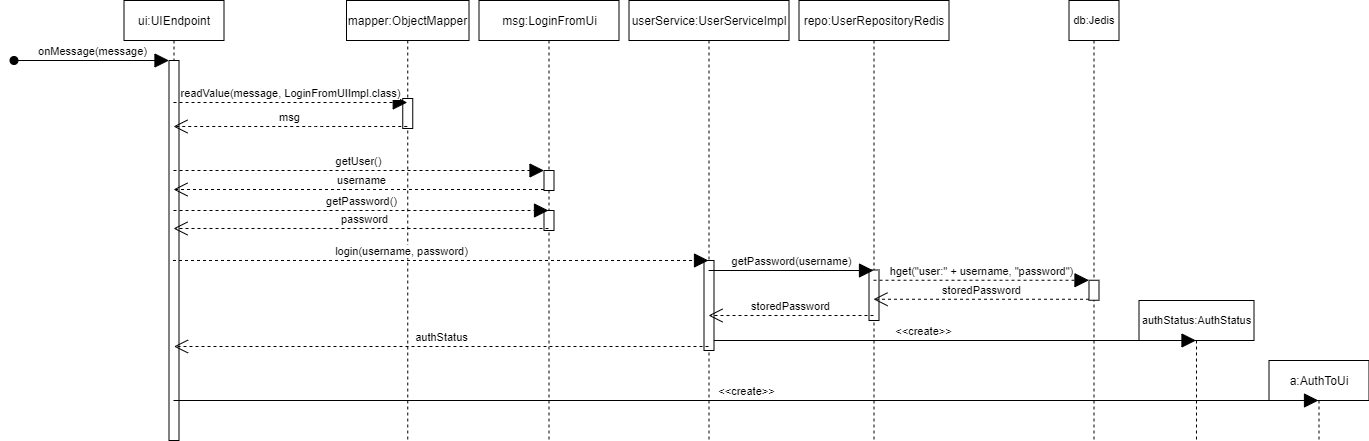
\includegraphics[width=25.7cm]{img/server_seq3.png}
        \caption{Server - UI richiede eliminazione unità}
    \end{figure}
\end{landscape}
